\section{Problembeskrivelse}
\label{sec:issue}

En dirac-puls $\delta(t)$ er et matematisk objekt som aldri kan realiseres fysisk. Det er en uendelig kort puls med uendelig stor verdi men som inneholder en endelig mengde eneregi.

Selv om dirac-pulsen ikke kan realiseres i praksis, har den en viktig teoretisk betydning. Dersom vi tenker oss at den utgjør inngangen til et lineært tidsinvariant system, vil utgangen av systemet $h(t)$, som vi kaller systemets impulsrespons inneholde all informasjon om systemets egenskaper. Se figur \ref{fig:01_problemstilling}.

\begin{figure}[!hbt]
	\centering
	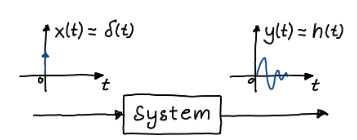
\includegraphics[]{./Images/01Issue/01.png}
	\caption{Når inngangen til et system har form av en dirac-puls $\delta(t)$, er utgangen per definisjon systemets impulsrespons $h(t)$.}
    \label{fig:01_problemstilling}
\end{figure}


En tilnærming til impulsresponsen kan man få ved å bruke som inngangssignal en uls av endelig, men veldig kort varighet og så registrere systemets respons. Et eksempel på en slik undersøkelse finner vi i rom-akustikken. Da man skulle vurdere plasseringen av Wagner-orgelet i Nidaros dom-kirke, ble det avfyrt pistol-skudd ulike steder i bygningen for å estimere rommets impulsrespons. For et elektronisk system kan impulresponsen undersøkes ved hjelp av en impuls-generator og et oscilloskop som vist i figur \ref{fig:02_problemstilling}.

\begin{figure}[!hbt]
	\centering
	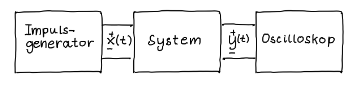
\includegraphics[scale=0.9]{./Images/01Issue/02.png}
	\caption{Undersøkelse av impulsrespons ved hjelp av impulsgenerator og oscilloskop.}
    \label{fig:02_problemstilling}
\end{figure}

Impulsgeneratoren produserer et signal $x(t)$ bestående av en serie korte pulser med avstand T. I det teoretisk ideelle tilfellet, består $x(t)$ av uendelig korte dirac-pulser som vist i figur \ref{fig:03_problemstilling}. Utgangen $y(t)$ av systemet avleses på oscilloskopet. 

\begin{figure}[!hbt]
	\centering
	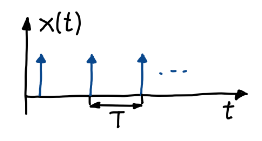
\includegraphics[scale=0.7]{./Images/01Issue/03.png}
	\caption{Sekvens av ideelle dirac-pulser.}
    \label{fig:03_problemstilling}
\end{figure}

En praktisk impulsgenerator vil generere korte pulser, jo kortere jo bedre. En design-ide for en slik impulsgenerator er som vist i figur \ref{fig:04_problemstilling}.

\begin{figure}[!hbt]
	\centering
	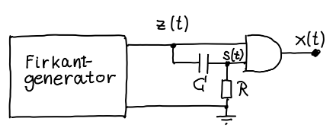
\includegraphics[scale=0.7]{./Images/01Issue/04.png}
	\caption{Ide til impulsgenerator.}
    \label{fig:04_problemstilling}
\end{figure}

Her blir signalet $z(t)$ sendt inn i høypassfilteret for å få ut signalet $s(t)$ der disse to signalene blir sendt inn i en AND gate for å så ut signalet $x(t)$ som er tilnermet en diracpuls $\delta (t)$. Signalene burde se noe tilsvarende figur \ref{fig:05_problemstilling}.

\begin{figure}[!hbt]
	\centering
	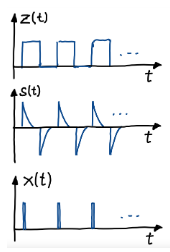
\includegraphics[scale=0.7]{./Images/01Issue/05.png}
	\caption{Signalformer som inngår i generator-ideen.}
    \label{fig:05_problemstilling}
\end{figure}

I dette designet skal ideen i figur \ref{fig:04_problemstilling} undersøkes og egenskapene testet.